\documentclass[12pt, 
hyperref={colorlinks=true, linkcolor=blue, urlcolor=cyan}]{beamer}
\usetheme{default} 

\setbeamertemplate{navigation symbols}{} %gets rid of navigation symbols
\setbeamertemplate{footline}{} %gets rid of bottom navigation bars
\setbeamertemplate{footline}[page number]{} %use this for page numbers

\setbeamertemplate{itemize items}[circle] %round bullet points
\setlength\parskip{10pt} % white space between paragraphs

\usepackage{wrapfig}
\usepackage{subfig}
\usepackage{setspace}
\usepackage{enumerate}
\usepackage{graphicx}
\usepackage{amsmath}
\usepackage{amsfonts}
\usepackage{amssymb}
\usepackage{amsthm}
\usepackage[UKenglish]{isodate}

\cleanlookdateon

% the preamble
\title{BIOST 311: \\ Regression Methods for the Health Sciences}
\author{Kelsey Grinde and Brian Williamson}
\institute{UW Biostatistics}
\date{26 March 2018}

\begin{document}
% title slide
\begin{frame}
\titlepage\thispagestyle{empty}
\end{frame}


% no chapter # for Day One chapter
\setbeamertemplate{footline}{%
  \raisebox{5pt}{\makebox[\paperwidth]{\makebox[120pt]{\scriptsize Last updated \today}\hfill\makebox[10pt]{\insertframenumber~~}}}}
\newcounter{day1}{\value{1}}
\setcounter{framenumber}{\value{day1}}

\begin{frame}
\frametitle{Welcome to BIOST 311!}

About this course:
\begin{itemize}
\item[] \textit{BIOST 311: Regression Methods for the Health Sciences} is about the use of regression methods to answer scientific questions, especially as related to the health sciences.
\end{itemize}

What is regression and why is it so important?
\begin{itemize}
\item ``A set of statistical processes for estimating the relationships among variables." -- Wikipedia
\item ``Everything is regression!" -- Scott Emerson, MD, PhD
\item \textit{Very} widely used in the health sciences (and other fields!)
\end{itemize}

\end{frame}

\begin{frame}
\frametitle{Goals for today}

\begin{itemize}
\item Introductions
\item Review syllabus
\item Motivate and briefly introduce regression
\end{itemize}

\end{frame}

% introductions
\begin{frame}
\frametitle{The Instructors}
\begin{itemize}
\item[] Kelsey Grinde \\ Graduate student, Department of Biostatistics \\ grindek@uw.edu 
\item[]
\item[] Brian Williamson \\ Graduate student, Department of Biostatistics \\ brianw26@uw.edu
\end{itemize}
% mention logistics of 2 instructors: alternate by topic (~ every 2 wks) who will be lecturing; will both attend every lecture/discussion section, both familiar with topics being discussed; 
\end{frame}

\begin{frame}
\frametitle{Introductions}
\begin{itemize}
\item Name
\item Major
\item Year
\item Why are you taking this course?
\end{itemize}
% start with instructors, then go around room
\end{frame}

% syllabus
\begin{frame}
\frametitle{Syllabus: The Basics}

Course Structure:
\begin{itemize}
\item 3 lectures and 1 discussion section per week
	\begin{itemize}
	\item Lecture: MWF, 12:30--1:20pm, SOCC 301
	\item Discussion: Tu, 10:30--11:20am, SOCC 301 (or HSL)
	\end{itemize}
\item Office hours: W, 2:00--4:00pm, HSB H657 (or by appt)
\end{itemize}

\small{\textit{Note: to get to H657, it's easiest to take the stairs/elevators up to Floor 6 from the Rotunda, then follow signs for ``Biostatistics."}}

\end{frame}

% canvas page
\begin{frame}
\frametitle{Syllabus: Course Website}

Our course website is located on Canvas (canvas.uw.edu). 

\color{blue} We will use this page a lot! \color{black} % sign up for notifications
\begin{itemize}
\item Posting course material: syllabus, lecture slides, assignments, optional reading, etc. % mention that there's no textbook
\item Submitting assignments
\item Communication: announcements, emails, discussion board
\end{itemize}

Let's take a \href{https://canvas.uw.edu/courses/1203588}{look}. % briefly explain organization

\textbf{Your homework for tonight:} familiarize yourself with this page, sign up for notifications.

\end{frame}

% course communication
\begin{frame}
\frametitle{Syllabus: Course Communication}

In Class: \vspace{-0.3cm}
\begin{itemize} 
\item Lectures (will not be recorded)
\item Course participation: ask questions, group discussion, activities, index cards, Poll Everywhere (\textbf{please bring paper and pen/pencil to every class})
\end{itemize}

Online: \vspace{-0.3cm}
\begin{itemize}
\item We'll use Canvas for announcements and emails
\item For questions about course content and homework: use the Canvas discussion board
	\begin{itemize}
	\item We will monitor regularly and reply within 24 hours
	\item \textit{We encourage you to answer one another's questions!}
	\end{itemize}
\item For questions of a personal nature or about your course project: email \textbf{both} instructors
\end{itemize}

\end{frame}

% first index card
\begin{frame}
\frametitle{Your first index card!}

Please write the following information on your index card (and hand in at the end of class):
\begin{itemize}
\item Name
\item Pronunciation guide
\end{itemize}

Example:
\begin{itemize}
\item Kelsey Grinde
\item Kel-see Grin-``D"
\end{itemize}

\end{frame}

% student responsibilities
\begin{frame}
\frametitle{Syllabus: Your Responsibilities}

\begin{itemize}
\item Read syllabus
\item Attend and participate in lectures \hfill (5\%) % participation measured by index cards/activities
\item Attend and participate in discussion sections \hfill (5\%) % participation measured by activities
\item Complete homeworks (7) \hfill (25\%)
\item Final group project \hfill (20\%) % will introduce tomorrow in discussion section
\item Midterm Exams (2) \hfill (10\% each)
\item Final Exam \hfill (25\%)
\end{itemize}

Final grades will be determined by converting percentages to 4-point scale. At minimum: 95--100\% = 3.9--4.0 (A), 90--95\% = 3.5--3.8 (A-), 65\% = 1.8 (C-).
\end{frame}

% joint responsibiliities
\begin{frame}
\frametitle{Syllabus: Joint Responsibilities}
\begin{itemize}
\item \textit{Classroom climate}: respectful and inclusive of all students, active participation, minimize distractions % to minimize distractions: people with laptops sit in back; for participation: bring notebook
\item \textit{Academic integrity}: cheating and plagiarism will not be tolerated; collaboration is encouraged, but assignments should be written in your own words.
\item \textit{Access and accommodations}: please communicate DRS accommodations to us at your earliest convenience
\end{itemize}

Concerns? Feedback? Let us know!
\begin{itemize}
\item We will also have someone visiting from the Center for Teaching and Learning for a mid-quarter check-in.
\end{itemize}
\end{frame}

% what to expect: statistics
\begin{frame}
\frametitle{What to expect: statistics}
\begin{itemize}
\item You will need light algebra and mathematical reasoning
	\begin{itemize}
	\item No calculus assumed
	\item We won't prove technical results
	\item Exams will not require any math beyond basic arithmetic (but you can bring a calculator)
	\end{itemize}
\item This course is a natural sequel to BIOST 310
	\begin{itemize}
	\item We'll review important concepts this week
	\item Please come talk to us if you're concerned! 
	\end{itemize}
\item We will learn how to build regression models, estimate parameters, and interpret coefficients
\item Applications will be primarily in public health or health sciences examples
\end{itemize}
\end{frame}

% what to expect: computing
\begin{frame}
\frametitle{What to expect: computing}
\begin{itemize}
\item We will learn basic statistical computing in \texttt{R}
\item You are \textit{not} expected to have a computing background
	\begin{itemize}
	\item We will demonstrate important functions in lectures and discussion sections
	\item We will provide helpful resources: templates for homework assignments, \texttt{R} code ``cheat sheet" with useful functions, video tutorials (as applicable), etc.
	\end{itemize}
\item \textbf{You will need access to a laptop during Discussion}
	\begin{itemize}
	\item UW has quarterly loans, if needed \begin{tiny} (\href{http://uwstlp.com/public/home}{http://uwstlp.com/public/home}) \end{tiny}
	\item Come see us if you need help setting this up
	\item You will \textit{not} generally need a laptop during lectures
	\end{itemize}
\end{itemize}

\textbf{Your homework for tonight:} download \texttt{R} and \texttt{R Studio}.

\end{frame}


% pause for questions
\begin{frame}
\center \Large Any Questions?
\end{frame}

% motivating example: FEV data
\begin{frame}
\frametitle{Why regression?}
Motivating example:
\begin{itemize} 
\item Observational study of lung function and smoking: 654 kids who came in for routine check-up at pediatric clinic
\item Information collected:
	\begin{itemize}
	\item Age (years)
	\item Forced Expiratory Volume, or FEV (liters per second) 
	\item Height (inches)
	\item Sex (M/F)
	\item Smoking habits (yes/no)
	\end{itemize}
\end{itemize}
\end{frame}

\begin{frame}
\frametitle{Why regression?} % FEV data
We can already answer some interesting questions using the tools you've learned in previous stats courses: 
\begin{itemize} 
\item In 2015, it was estimated that 15\% of US adults were smokers. Is smoking less likely among children? 
	\begin{itemize}
	\item \textbf{One-sample test of proportion} ($H_0: p_0 = 0.15$)
	\end{itemize}
\item Are girls and boys equally likely to smoke?
	\begin{itemize}
	\item \textbf{Two-sample test of proportions} ($H_0: p_{boys} = p_{girls}$) \\ \textbf{Chi-squared test of independence} ($H_0:$ sex and smoking habits are independent)
	\end{itemize}
\item Does the average FEV differ between smokers and non-smokers?
	\begin{itemize}
	\item \textbf{Two-sample t-test} ($H_0: \mu_{smokers} = \mu_{nonsmokers}$)
	\end{itemize}
\end{itemize}
\end{frame}

\begin{frame}
\frametitle{Why regression?} % FEV data
What about other types of questions?
\begin{itemize} 
\item E.g., is age associated with FEV?
\end{itemize}
How would you assess this?
\begin{itemize}
\item Could divide age into pre-teens ($< 13$) and teens ($\ge 13$) 
\item Two-sample t-test (difference in average FEV between the two age groups): $H_0: \mu_{teen} = \mu_{preteen}$
\end{itemize}
\end{frame}

\begin{frame}
\frametitle{Example: Age and FEV} % FEV data
\center 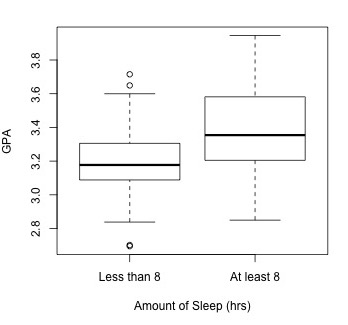
\includegraphics[height=0.9\textheight]{./intro_boxplot} % boxplot of age grp vs FEV
\end{frame}

\begin{frame}
\frametitle{Example: Age and FEV} % FEV data
The question is: why regression?
\begin{itemize}
\item What if we wanted to understand how children differ in their lung capacity (FEV) across different levels of age (not just two categories, but on a continuous scale?)
\end{itemize}
\end{frame}

\begin{frame}
\frametitle{Example: Age and FEV} % FEV data
\center 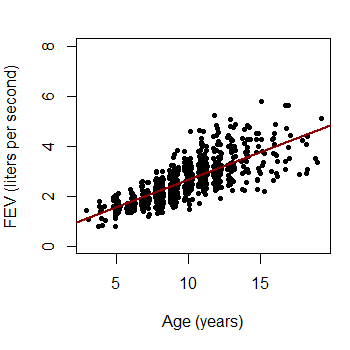
\includegraphics[height=0.9\textheight]{./intro_scatterplot} %scatterplot of age vs FEV; why isn't this the same as the dataset we used on our poster?????
\end{frame}

\begin{frame}
\frametitle{Why regression?} 
Linear regression
\begin{itemize}
\item In BIOST 310, you learned about linear regression to answer questions like this
	\begin{itemize} 
	\item E.g., age and FEV
	\item \textbf{Can also adjust for other variables} (e.g., smoking) % like our course poster!
	\end{itemize}
\item (Approximately three weeks of our course will cover linear regression and we will go into much more detail than in BIOST 310)
\end{itemize}
\end{frame}

\begin{frame}
\frametitle{Why regression?}
Other types of outcomes:
\begin{itemize}
\item What if your outcome is a simple yes/no?
	\begin{itemize}
	\item Smoker or non-smoker?
	\item Diabetes or no diabetes?
	\item Death or no death?
	\end{itemize}
\item What if your outcome is a time-to-event, in which not everyone achieves that event?
	\begin{itemize}
	\item Time to promotion?
	\item Time to cancer remission?
	\item Time to death?
	\item Age at which you start smoking? % this work?
	\end{itemize}
\end{itemize}

Later in the course, we'll learn about other types of regression that are often useful in these settings.
\end{frame}

% puase for questions
\begin{frame}
\center \Large Any Questions?
\end{frame}

% What's next?
\begin{frame}
\frametitle{Tentative schedule moving forward...}
\begin{itemize}
\item Chapter 0: BIOST 310 review \hfill 3/28--4/2
\item Chapter 1: linear regression \hfill 4/4--4/27
\item Chapter 2: logisitic regression \hfill 4/30--5/11
\item Chapter 3: proportional hazards regression \hfill 5/14--5/21
\item Chapter 4: special topics \hfill 5/23--5/30
\item Final review and exam \hfill 6/1 \& 6/7
\end{itemize}
\end{frame}


% make it 0. something (for Chapter 0)
%\setbeamertemplate{footline}{%
  %\raisebox{5pt}{\makebox[\paperwidth]{\makebox[120pt]{\scriptsize Last updated \today}\hfill\makebox[10pt]{\scriptsize 0.\insertframenumber~~}}}}  \newcounter{chap0}{\value{1}}
%\setcounter{framenumber}{\value{chap0}}
%\begin{frame}
%\frametitle{CHAPTER 0: REVIEW OF BIOST 310}
%\end{frame}

% make it 1. something (for Chapter 1)
%\setbeamertemplate{footline}{%
  %\raisebox{5pt}{\makebox[\paperwidth]{\makebox[120pt]{\scriptsize Last updated \today}\hfill\makebox[10pt]{\scriptsize 1.\insertframenumber~~}}}}  \newcounter{chap1}{\value{1}}
%\setcounter{framenumber}{\value{chap1}}
%\begin{frame}
%\frametitle{CHAPTER 1: LINEAR REGRESSION}
%\end{frame}

% For tomorrow:
\begin{frame}
\frametitle{For tomorrow:}

\begin{itemize}
\item Download \texttt{R} and \texttt{R Studio} (see instructions on Canvas)
\item Meet in Health Sciences Library computer lab tomorrow morning (Classroom C); bring your laptop
\item Start working on:
	\begin{itemize}
	\item Familiarizing yourself with Canvas page and Syllabus
	\item HW1 (due Friday)
	\end{itemize}
\end{itemize}

\end{frame}

\end{document}
